\documentclass[a4paper]{article}
\usepackage[dutch]{babel}
\usepackage{amsthm,amsmath}
\usepackage{graphicx}
\usepackage{epstopdf}
\usepackage{enumerate}
\usepackage{amssymb}
\usepackage{float}
\usepackage{algpseudocode}
\usepackage{varwidth}
\usepackage{mcode}
\usepackage{algorithm}


\title{Practicum NMB : Eigenwaardenproblemen}
\author{Jona Beysens \& Arnout Devos}
\date{vrijdag 25 apil 2014}

\newcommand{\opgave}[1]{\section*{Opgave #1}}
\newcommand{\dx}{\Delta x}
\newcommand{\dy}{\Delta y}
\newcommand{\dz}{\Delta z}
\newcommand{\dt}{\Delta t}

\begin{document}
\maketitle

\opgave{1}

\begin{algorithm}
 \label{alg:alg1}
 \caption{Aangepaste gelijktijdige iteratie}
\begin{algorithmic}[1]
\State Kies $Q^{(0)} \in \mathbb{R}^{m\times d}$ met orthonormale kolommen.
\For {$k = 1,2,...$}
    \State $AZ=Q^{(k-1)}$
    \State $Q^{(k)}R^{(k)}=Z$
    \State $A^{(k)}=Q^{(k)^{T}}AQ^{(k)}$
\EndFor
\State $x = 1./diag(A^{(k)})$
\end{algorithmic}
\end{algorithm}
\ \\
Dit algoritme is de gelijktijdige inverse iteratie voor het berekenen van de d kleinste eigenwaarden en bijhorende eigenvectoren van de matrix $A$. Het is een aangepaste versie van de gelijktijdige iteratie waarbij gebruik gemaakt wordt van de inverse van $A$. De inverse wordt echter nooit expliciet berekend maar er wordt telkens een stelsel opgelost naar $Z$. De eigenwaarden van $A^{-1}$ zijn de inversen van de eigenwaarden van $A$ en de eigenvector horende bij $\lambda_i$ is dezelfde als die horende bij $\frac{1}{\lambda_i}$:
\begin{proof}
\begin{align}
	Ax &= \lambda x \label{eq1}\\ 
    A^{-1}Ax &= \lambda A^{-1}x \label{eq2}\\
    \frac{1}{\lambda}x &= A^{-1}x \label{eq:const1}
\end{align}
\end{proof}
De eigenvectoren horende bij de kleinste eigenwaarden van $A$ komen nu in de eerste kolommen van $Q$ te staan. Daardoor zal $A^{(k)}$ convergeren naar een diagonaalmatrix waarvan de eerste diagonaalelementen de kleinste eigenwaarden van $A$ zijn.

\opgave{2}
\begin{enumerate}[a)] % a), b), c), ...
\item Als $\mu$ een eigenwaarde van $A$ goed benadert, worden de grootste eigenwaarde van $(A-\mu I)^{-1}$ en het conditiegetal van $(A-\mu I)$ zeer groot. Daardoor zal bij het aanleggen van een willekeurige perturbatie op de matrix $(A-\mu I)$ de oplossing $\hat{y}$ van het stelsel sterk afwijken van het originele probleem. Omdat de perturbatie willekeurig is, zal de resulterende verandering in elke richting even sterk optreden. Hierdoor zullen de resulterende eigenvectoren slechts weinig verschillen van de originele. De grootste eigenwaarde is zo dominant dat de oplossing van het geperturbeerd probleem $\hat{y}$ bijna in dezelfde richting ligt als $y$. De grootte van $\hat{y}$ verschilt echter sterk van deze van $y$. De perturbatie wordt sterk uitvergroot. Door te normaliseren verschillen $\hat{y}$ en $y$ enkel nog in richting. Dit verschil is miniem.
\item Om het residu van $Ax-\rho x$ te minimaliseren lossen we het kleinste kwadratenprobleem op:
\begin{proof}
\begin{align}
\displaystyle\min_{\rho\in\mathbb{R}}\Arrowvert Ax-\rho x \Arrowvert _2 \Leftrightarrow x^{T}(Ax-x\rho) &= 0\label{eq1}\\
 x^TAx &= x^T\rho x \label{eq2}\\
 \rho&=\frac{x^TAx}{x^Tx} \label{eq:const1}
\end{align}
\end{proof}
Deze oplossing voor $\rho$ komt overeen met het Ragleigh quoti\"{e}nt $r(x)$.
\end{enumerate}



\opgave{3}
Voor beide oefeningen worden \textit{Rayleigh inverse iteratie} en \textit{QR algoritme met shifts} verkozen boven de anderen. De maximale convergentiesnelheid van deze methodes is kubisch. Bovendien is hun rekenkost aanvaardbaar. \textit{Power iteratie}, \textit{Inverse iteratie zonder shift} en \textit{QR algoritme zonder shift} leveren slechts lineaire convergentie op. Daarom worden deze niet verder in rekening gebracht. 
\begin{enumerate}[a)] % a), b), c), ...
\item 
Aangezien er een schatting voor de eigenvector gegeven is, is de \textit{Rayleigh inverse iteratie} een geschikte methode om de bijhorende eigenwaarde te vinden. Er dient maar 1 eigenwaarde berekend te worden. 

Deze methode zal bovendien zorgen voor snelle convergentie. De verwachte convergentiesnelheid is immers maximaal kubisch. Dit wordt aangetoond in \textbf{Theorema 27.3 Trefethen and Bau}. 

Om de rekenkost van de iteratie te beperken wordt de symmetrische matrix $A \in \mathbb{R}^{m\times m}$ getransformeerd tot een tridiagonale matrix. Hiervoor wordt Householder triangularisatie gebruikt. In het algemeen bedraagt totale hoeveelheid rekenwerk hiervoor  $\frac{10m^{3}}{3}$ flops. Aangezien gebruikt gemaakt kan worden van symmetrie en spaarsheid kan dit werk gereduceerd worden tot $\frac{4m^{3}}{3}$ flops. 

In elke stap van de \textit{Rayleigh inverse iteratie} wordt een stelsel opgelost. Dit zorgt voor het meeste werk in elke stap. Dit vraagt in het algemeen $\mathcal{O} (m^3)$ flops. Door gebruik te maken van een vereenvoudigde vorm van Gaussiaanse eliminatie (\textit{Thomas algoritme}) kan het rekenwerk gereduceerd worden tot $\mathcal{O}(m)$ flops. Ook wordt de oplossing van het stelsel genormaliseerd. Dit vraagt $n$ flops. Als laatste wordt het \textit{Rayleigh quoti\"ent} berekend. $Av$ zorgt ongeveer voor $5n$ flops (maximaal 3 vermenigvuldigingen en 2 optellingen per element). $v^{T}Av$ kost dan uiteindelijk nog $2n-1$ flops($n$ vermenigvuldigingen en $n-1$ optellingen). \textit{Rayleigh quoti\"ent} vraagt dus ongeveer $7n-1$ flops. Als we ervan uitgaan dat convergentie bereikt wordt in $\mathcal{O}(m)$ stappen bedraagt het totale rekenwerk na de tridiagonalisatie dus globaal $\mathcal{O} (m^2)$.

\item
Om de eigenwaarde te bepalen die zich het dichtst bij een getal $\alpha$ bevindt, is het \textit{QR algoritme met shifts} een geschikte methode. Er is namelijk geen benadering voor een eigenvector gegeven, wat voor de \textit{Rayleigh inverse iteratie} wel noodzakelijk is (al zouden we een willekeurige startvector kunnen kiezen). Het \textit{QR algoritme met shifts} berekent alle eigenwaarden. Hierdoor kunnen we makkelijk zien hoe ver de minder dichte eigenwaarden zich van $\alpha$ bevinden. We kunnen $\alpha$ als initi\"ele benadering voor de te zoeken eigenwaarde gebruiken. In elke iteratie verbeteren we de benadering door het Rayleigh quoti\"ent te nemen. 

Het \textit{QR algoritme met shifts} convergeert maximaal kubisch naar de gezochte eigenwaarde. Het convergeert lineair naar de andere eigenwaarden. 

Om het rekenwerk te verminderen (zie opgave 4), is ook hier tridiagonalisatie van $A$ vereist. Dit vergt  $\frac{4m^{3}}{3}$ flops (zie a). In elke stap van het algoritme moet een QR factorisatie berekend worden. De vector $v$ die nodig is voor het berekenen van de Householder reflector heeft slechts 2 elementen verschillend van 0. Het opstellen van van de reflector vraagt ongeveer $20n$ flops (2 normen en een deling). Bij het toepassen van de reflectoren op de matrix A worden er door elke reflector maximaal 5 elementen aangepast. Hiervoor zijn 3 flops per element nodig (2 vermenigvuldigingen en 1 optelling).Dit levert dus 15 flops in totaal per reflector. Na $n-1$ reflectoren wordt de bovendriehoeksmatrix bekomen dus in totaal zijn er ongeveer $15(n-1)$ flops vereist. 

Ook moet er in elke stap van het algoritme $RQ$ berekend worden. Ook deze bewerking vraagt $\mathcal{O}(m)$ rekenwerk omdat hier de householder reflectoren kunnen gebruikt worden om het product uit te rekenen. Indien convergentie in $\mathcal{O}(m)$ stappen gebeurt, zal ook deze methode buiten de tridiagonalisatie in totaal $\mathcal{O} (m^2)$ rekenwerk vragen. Merk op dat er bij deze berekening van de rekenkost geen rekening gehouden werd met het bijhouden van de geaccumuleerde eigenvector matrix $Q$. Er werd immers geen eigenvector gevraagd in de opgave.
\end{enumerate}
\opgave{4}
In figuur ~\ref{fig:figure1} zien we de structuur van de matrix \textit{mat1.txt} na reductie naar de Hessenberg vorm. Doordat de matrix niet perfect symmetrisch is, staan er nog waarden in de bovendriehoek die verschillend zijn van 0. Als we kijken naar de grootte van de waarden in die bovendriehoek dan zijn deze allemaal klein. Als we alle waarden die in absolute waarde kleiner dan $10^{-14}$ zijn gelijk aan 0 stellen dan verkrijgen we de vorm in figuur ~\ref{fig:figure2}. Deze tridiagonale vorm is typisch voor reductie van een symmetrische matrix naar een Hessenberg vorm.

Indien de matrix niet gereduceerd zou worden naar Hessenberg vorm, moet in elke iteratie van het QR algoritme de factorisatie berekend worden van een volle matrix. Dit vergt $\mathcal{O}(m^{3})$ flops. De convergentie naar machinenauwkeurigheid $\epsilon _{mach}$ gebeurt meestal in $\mathcal{O}(m)$ stappen wat het totale vereiste werk op $\mathcal{O}(m^{4})$ flops brengt. Het rekenwerk van de QR factorisatie van een matrix in Hessenbergvorm bedraagt $\mathcal{O}(m^{2})$ flops. Hierdoor komt het totale werk op $\mathcal{O}(m^{3})$ flops. Aangezien de Hessenbergvorm van de matrix $mat1.txt$ een tridiagonale vorm heeft zal er zelfs nog minder werk nodig zijn. Het rekenwerk voor een QR factorisatie van een tridiagonale matrix is immers $\mathcal{O}(m)$ flops waarmee het totale rekenwerk op $\mathcal{O}(m^{2})$ flops komt.
\begin{figure}[H]
\begin{minipage}[t]{0.45\linewidth}
\centering
\centerline{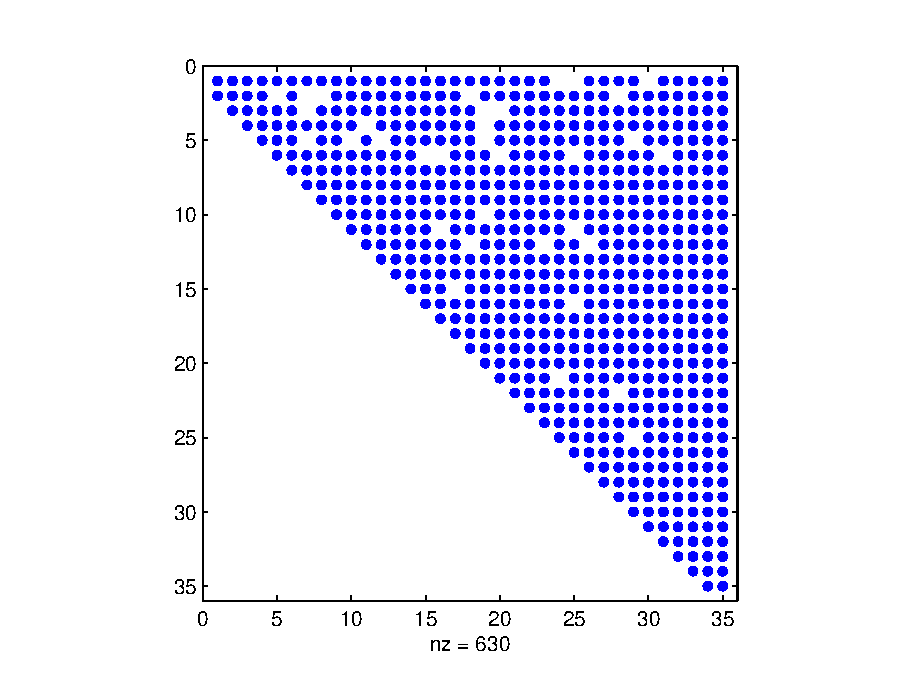
\includegraphics[scale=0.45]{pictures/opgave4Hessenberg1.eps}}
\caption{Vorm van de matrix \textit{mat1.txt} door reductie naar Hessenberg vorm}
\label{fig:figure1}
\end{minipage}
\hfill
\begin{minipage}[t]{0.45\linewidth}
\centering
\centerline{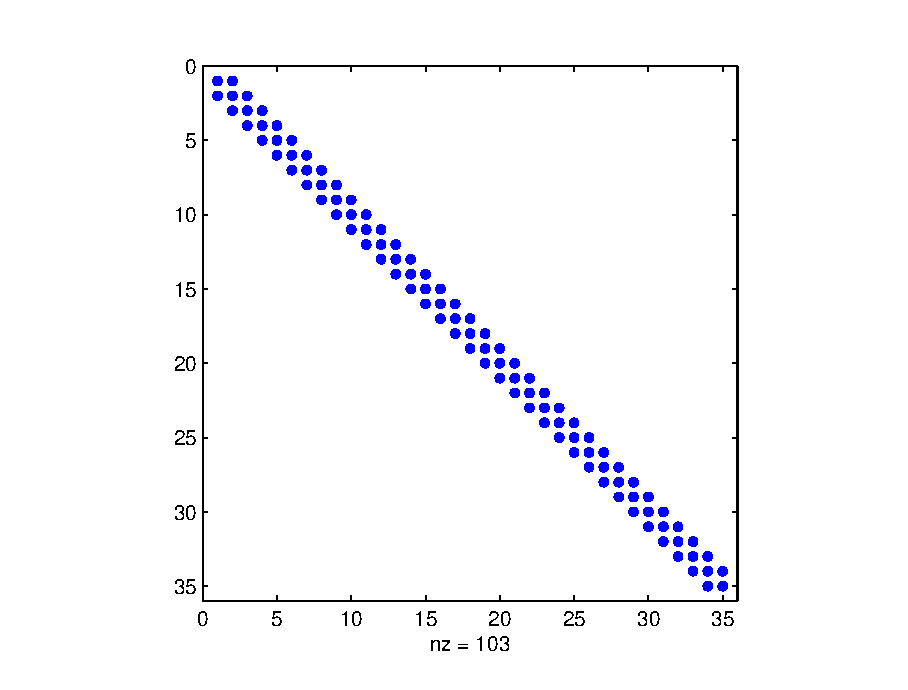
\includegraphics[scale=0.45]{pictures/opgave4Hessenberg2.eps}}
\caption{Tridiagonale vorm van de matrix \textit{mat1.txt} na reductie naar Hessenberg vorm en verwaarlozing van elementen $<10^{-13}$}
\label{fig:figure2}
\end{minipage}
\end{figure}
\opgave{5}
Op figuur ~\ref{fig:opgave5} kunnen we duidelijk zien dat de \textit{QR-methode zonder shift} lineair convergeert wat overeenkomt met de theorie.
\begin{figure}
\centerline{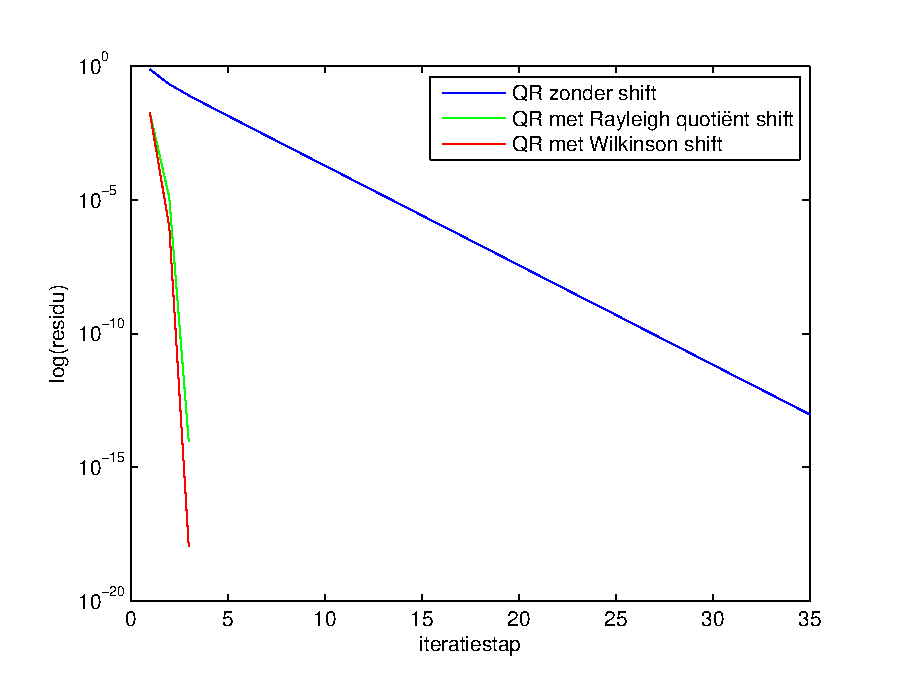
\includegraphics{pictures/opgave5grafiek.eps}}
\caption{Convergentie van de verschillende QR methodes: zonder shift, Rayleigh quoti\"{e}nt shift en Wilkinson shift op logaritmische schaal.}
\label{fig:opgave5}
\end{figure}
In tabel \ref{table:tab2} zien we dat voor de matrix mat1 er voor de \textit{QR iteratie met Rayleigh quoti\"{e}nt shift} en de \textit{QR iteratie met Wilkinson shift} er eerst lineaire convergentie optreedt. Wanneer bij deze algoritmes het residu voldoende klein is geworden, verloopt de convergentie meer en meer kubisch. Dit komt overeen met de theorie die zegt dat $q_m^{(k)}$ kubisch convergeert tot een eigenvector. Daardoo convergeert ook het bijbehorende Rayleigh quoti\"{e}nt $r(q_m^{(k)})=A_{mm}^{(k)}$ kubisch. Naarmate het aantal iteraties toeneemt wordt de invloed van de kubische convergentie steeds groter omdat het aantal elementen dat nog moet convergeren naar een eigenwaarde in elke iteratiestap kleiner wordt.
\begin{table}[h]
\begin{tabular}{|l|l|l|l|}
\hline
stap & zonder shift & Rayleigh quoti\"{e}nt shift & Wilkinson shift \\
\hline
1 & 0.763590501238868 & 0.0183598152348892 & 0.0183598152348892 \\
2 & 0.210113423731095 & 1.23415266649239e-05 & 9.83319921427331e-07 \\
3 & 0.0808375414586785 & 9.55801949807706e-15 & 1.13833614396543e-18 \\
\vdots & \vdots &  &  \\
10 & 0.000192468492953297 &  &  \\
11 & 8.16489243297394e-05 &  &  \\
12 & 3.46381851762602e-05 &  &  \\
13 & 1.46948586913677e-05 &  &  \\
14 & 6.23416040757481e-06 &  &  \\
15 & 2.64479155115201e-06 &  &  \\
16 & 1.12203213434041e-06 &  &  \\
\vdots & \vdots &  &  \\
32 & 1.23546560557316e-12 &  &  \\
33 & 5.24136923576435e-13 &  &  \\
34 & 2.22361119093024e-13 &  &  \\
35 & 9.43350202212816e-14 &  &  \\
\hline
\end{tabular}
\caption{Convergentie van het residu bij de berekening van eigenwaarden volgen verschillende methodes.}
\label{table:tab2}
\end{table}
\opgave{6}
Het verband tussen het \textit{QR-algoritme met Rayleigh quoti\"{e}nt shift} en de \textit{Rayleigh quoti\"{e}nt iteratie}, is dat de veronderstelde waarden voor de eigenvector
en eigenwaarde bij het QR-algoritme, $q_m^{(k)}$ en $\mu$ respectievelijk, dezelfde zijn als de waarden
die berekend worden bij de Rayleigh quoti\"{e}nt iteratie met startvector $e_m$. Er wordt dus een Rayleigh quoti\"{e}nt iteratie toegepast op de laatste eigenwaarde van
A. De Rayleigh quoti\"{e}nt iteratie convergeert kubisch, dus de convergentie van het QR algoritme met Rayleigh shift moet ook kubisch zijn. De Rayleigh shift heeft geen invloed op de andere eigenwaarden, dus er wordt verwacht dat deze lineair convergeren net als bij gelijktijdige iteratie het geval is. Dit is te zien in Figuur ~\ref{fig:opgave6}.
\begin{figure}
\centerline{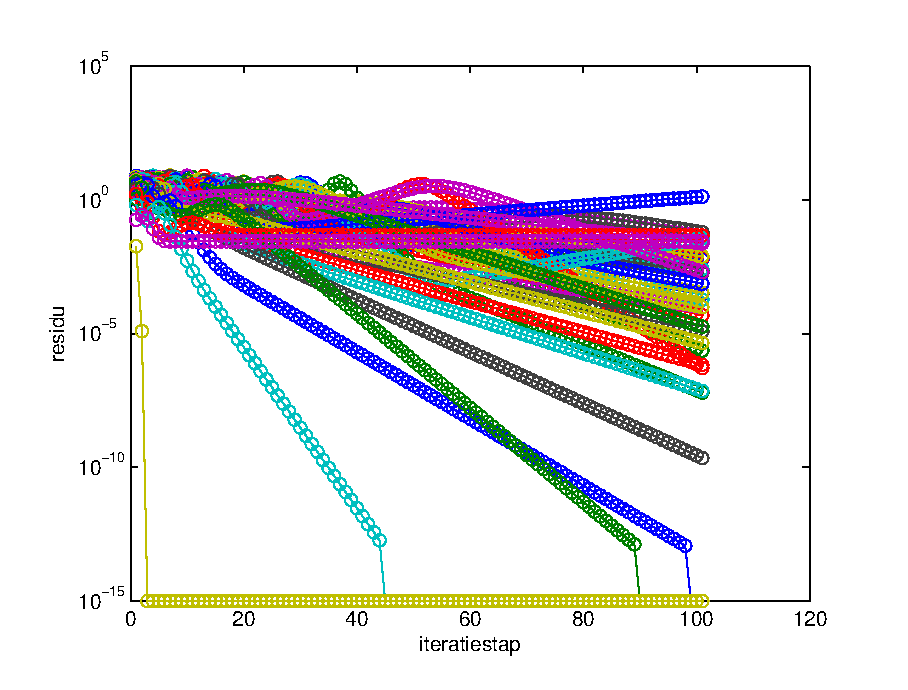
\includegraphics{pictures/opgave6.eps}}
\caption{Convergentie van de norm van de subdiagonale elementen van matrix $mat1$ in het QR algoritme met Rayleigh quoti\"{e}nt shift}
\label{fig:opgave6}
\end{figure}
\opgave{7}
Als men de \textit{Arnoldi} methode gebruikt op een ijle matrix $A \in \mathbb{R}^{1000\times1000}$ en de Ritz waarden per iteratiestap uitzet dan verkrijgt men Figuur ~\ref{fig:opgave7}.
Wat opvalt aan het convergentiegedrag is dat er eerst snelle convergentie optreedt naar de grootste eigenwaarde. Wanneer de Ritz waarde in de buurt komt van deze eigenwaarde,wordt de fout tussen de Ritz waarde en de eigenwaarde enkel nog kleiner. Vroege convergentie is te zien aan de lange rode lijnen die niet meer afwijken van een bepaalde waarde. Het convergentiegedrag is lineair en versnelt wanneer er meer eigenwaarden gevonden zijn.
\begin{figure}
\centerline{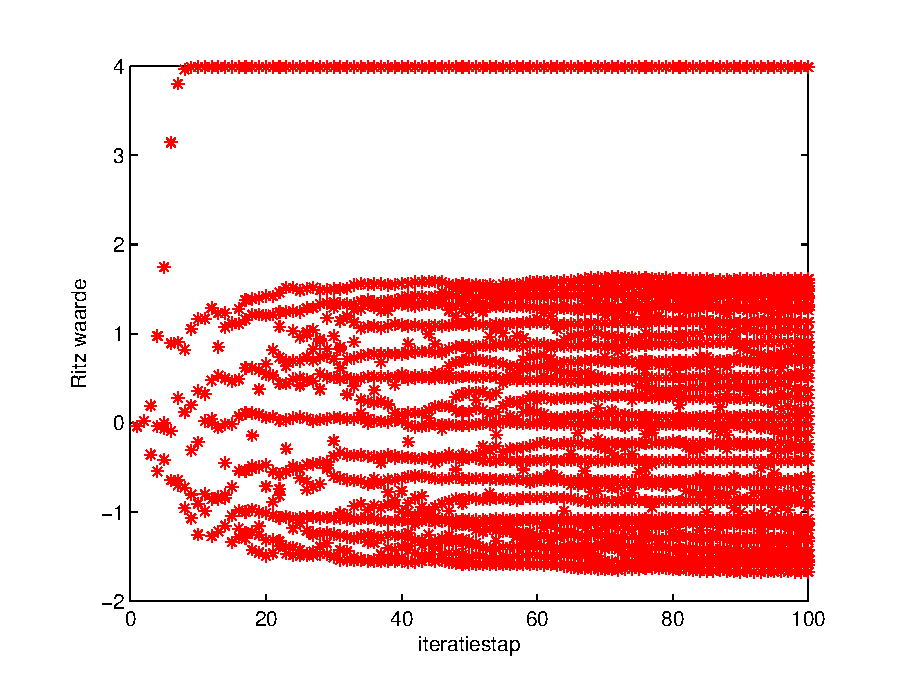
\includegraphics{pictures/opgave7arnoldiBeter.eps}}
\caption{Convergentie van de Ritz waarden naar de eigenwaarden van A.}
\label{fig:opgave7}
\end{figure}

\opgave{8}
\begin{algorithmic}
\State
\begin{align*}
&J^{T}
\begin{bmatrix} 
a & d \\
d & b 
\end{bmatrix}
J
=
\begin{bmatrix} 
\neq 0 & 0 \\
0 & \neq 0
\end{bmatrix}\\
&\begin{bmatrix} 
c & -s \\
s & c
\end{bmatrix}
\begin{bmatrix} 
a & d \\
d & b 
\end{bmatrix}
\begin{bmatrix} 
c & s \\
-s & c 
\end{bmatrix}
=
\begin{bmatrix} 
\neq 0 & 0 \\
0 & \neq 0
\end{bmatrix}\\
&\Leftrightarrow d.(c^2-s^2)+(a-b).c.s = 0 \\
 &\Leftrightarrow d. cos(2\theta)+(a-b) \frac{sin(2\theta)}{2}= 0\\
 &\Leftrightarrow \frac{sin(2\theta)}{cos(2\theta)} = \frac{2.d}{b-a}\\
 &\Leftrightarrow tan(2\theta) = \frac{2.d}{b-a}
\end{align*}

\end{algorithmic}
\opgave{9}
De code in Matlab bevindt zich hieronder. De pseudocode bevindt zich in bijlage.
\lstinputlisting{jacobi.m}


\begin{table}[h]
\begin{tabular}{|l|l|}
\hline
stap & 2-norm van niet-diagonaal elementen\\
\hline
1 & 1.969312339842242e+01\\
2 & 7.532976092556866e+00\\
3 & 2.243630988647221e+00\\
4 & 4.492085536126931e-01\\
5 & 1.037550717669171e-02\\
6 & 3.073093957017962e-05\\
7 & 8.022616206681419e-11\\
8 & 1.988610766134013e-14\\
\hline
\end{tabular}
\caption{Convergentie de norm van de niet-diagonaal elementen van de matrix D naar 0 bij een opgegeven $tol =10^{-13}$.}
\label{table:tab2}
\end{table}
\opgave{10}
Om de eigenwaarden tot op een nauwkeurigheid van $10^{-13}$ te berekenen convergeert het algoritme in 8 stappen. Als stopconditie wordt de 2-norm van de niet-diagonaal elementen gebruikt. Deze wordt berekend als volgt: $\epsilon = \sqrt[2]{\mathop{\sum\sum}_{t\neq u} D(t,u)^2}$. Hierbij stelt $D$ de matrix voor waarop de jacobi iteratie toegepast wordt in elke stap. Opdat deze stopconditie de juiste resultaten zou leveren, wordt $\epsilon$ vergeleken met de relatieve fout op de eigenwaarden van $A$ (zie figuur~\ref{fig:figure 3}). Uit deze figuur blijkt dat de convergentie van de eigenwaarden van $D$ naar die van $A$ even snel gebeurt als de convergentie van $\epsilon$ naar 0. Meer nog, de fout op de eigenwaarden is steeds ongeveer $10^{-2}$ kleiner dan $\epsilon$. Dus als we $\epsilon$ tot op een nauwkeurigheid van \textit{tol} berekenen, zullen de eigenwaarden minstens even nauwkeurig zijn. Er wordt dus steeds voldoende werk geleverd.

In theorie is de convergentiesnelheid van de methode van Jacobi meer dan lineair en maximal kwadratisch. In praktijk zien we hetvolgende (zie tabel~\ref{table:tab2}): tot de 4e stap is er lineaire convergentie. Hierna verdubbelt het aantal juiste beduidende cijfers in elke stap. Deze kwadratische convergentie kan ook gezien worden in figuur~\ref{fig:figure 3}: de helling van de fout steeds toe (meer negatief).

De rekenkost is de volgende: elke stap worden er door $D$ rechts te vermenigvuldigen met $J$ twee kolommen aangepast. Dit vergt $3m$   flops per kolom. Ook wordt $D$ links vermenigvuldigd met $J^{T}$.  Dit zorgt voor een aanpassing van twee rijen van A en vraagt $3m$ flops per rij. In elke stap is er dus $6m$ flops rekenwerk. In de volgende stap gaan de huidig gemaakte nullen verloren maar de amplitude van elementen wordt wel kleiner. Hierdoor kan er convergentie optreden. Bij een standaard rij per rij ordening wordt er in elke “sweep” $\frac{m(m-1)}{2}$ keer het product $J^{T}D J$ berekend waardoor het totale rekenwerk van een “sweep” $\mathcal{O}(m^{3})$ is. Bij kwadratische convergentie zijn er dus in totaal $\mathcal{O}(m^{3}log(|log(\epsilon_{machine})|)$ flops noodzakelijk.


\begin{figure}
\centerline{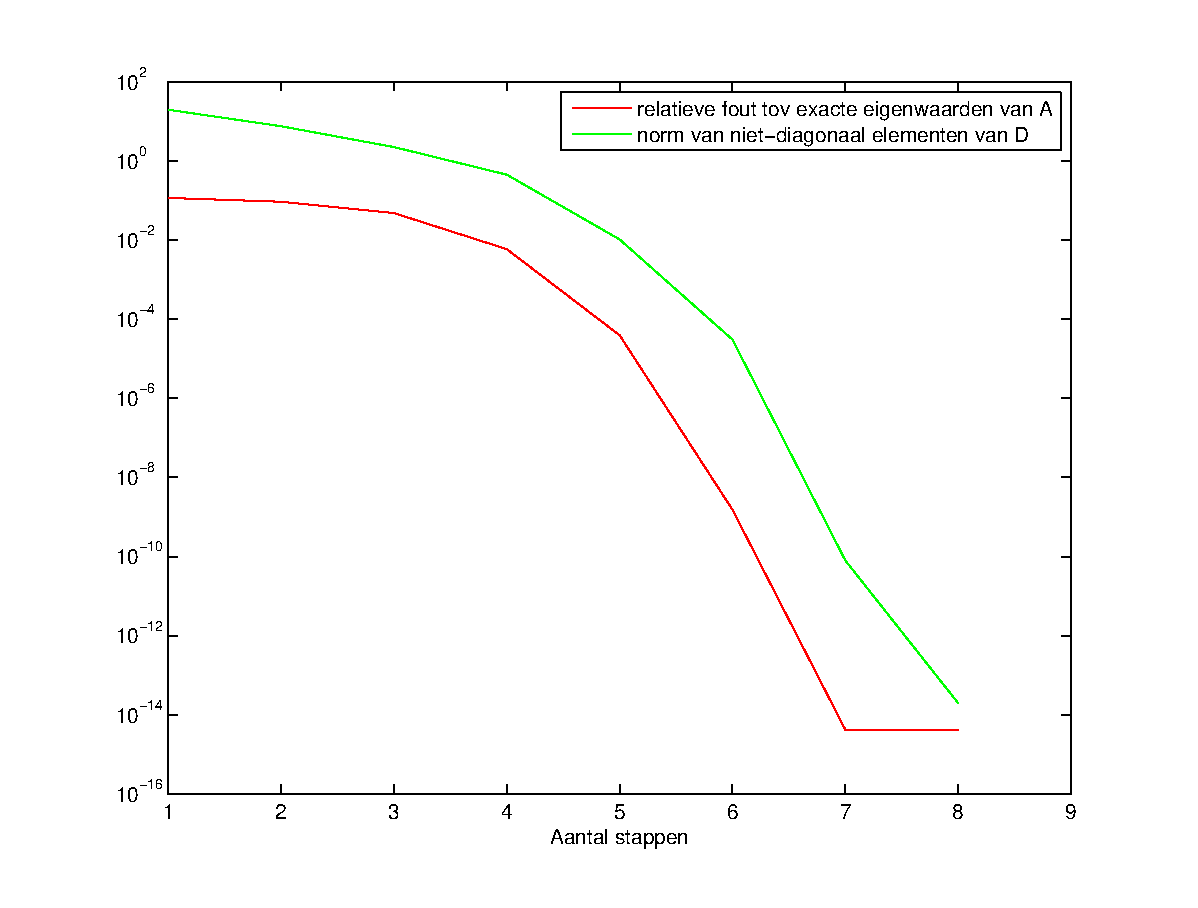
\includegraphics{pictures/opgave10.eps}}
\caption{Convergentie van de 2-norm van de subdiagonale elementen van matrix $mat1$ in het QR algoritme met Rayleigh quoti\"{e}nt shift}
\label{fig:figure 3}
\end{figure}

 \begin{algorithm}
 \caption{Jacobi Iteratie}
\begin{algorithmic}[1]
\State Stel $V \leftarrow I \in \mathbb{R}^{m\times m}$ \ \ \ \ {$V$ zal na de iteratie de eigenvectoren van $A$ bevatten.}
\State Stel $D^{(0)} \leftarrow A \in \mathbb{R}^{m\times m}$
\For {$k \leftarrow 1,2,...$} \ \ \ \ \ \ \ \ \ \ \ \ \ \ \ {Zolang $\epsilon >= tol$ zal iteratie blijven doorgaan.}
\For {$p \leftarrow 1$ to $m$}
\For {$q \leftarrow p$ to $m$}
\State $\theta \leftarrow \dfrac{Bgtan\dfrac{2D^{(k-1)}(p,q)}{D^{(k-1)}(q,q)-D^{(k-1)}(p,p)}}{2}$
\State Kies $J^{(k)}$ zodat
\State $J^{(k)} \leftarrow \begin{bmatrix} 
cos(\theta) & sin(\theta) \\
-sin(\theta) & cos(\theta)
\end{bmatrix}$
\State $D^{(k)} \leftarrow J^{T}DJ$
\State $V \leftarrow V J^{(k)}$
\State $\epsilon \leftarrow \sqrt[2]{\mathop{\sum\sum}_{t\neq u} D^{(k)}(t,u)^2}$ \ \ {2-norm van niet-diagonaal elementen.}
\EndFor
\EndFor
\EndFor
\end{algorithmic}
\label{alg:alg2}
\end{algorithm}


\end{document}